
\documentclass[10pt,letterpaper]{article}

\usepackage{hyperref}
\usepackage{cogsci}
\usepackage{pslatex}
\usepackage{pdfsync}
\usepackage{amsmath}
\usepackage{graphicx}
\usepackage{topcapt}
\usepackage{color}
\usepackage[english]{babel}



\title{Large scale investigations of variability in early language production}
\author{{\large \bf Rose M. Schneider} \\ \texttt{rschneid@stanford.edu}\\ Department of Psychology \\ Stanford University \\ 
\And {\large \bf Dan Yurovsky} \\ \texttt{yurovsky@stanford.edu} \\ Department of Psychology \\ Stanford University \\ 
\And {\large \bf Michael C. Frank} \\ \texttt{mcfrank@stanford.edu} \\ Department of Psychology \\ Stanford University \\ }

\begin{document}
\maketitle


%ABSTRACT
\begin{abstract}
The first word, an intimate moment between child and caretaker, exhibits a tremendous amount of variability in semantic categorization, phonological complexity, and age of onset. Through several large datasets of parental report of children's first words, we investigate patterns in first word production, including the age of onset, distribution of MB-CDI categories, and first words in relation to parental input and phonological complexity. In three analyses, we explore the timecourse and distribution of children's first recognizable language productions. We find that, contra conventional wisdom, more than 75 percent of children in our datasets produce a first word by their first birthday. In our second analysis, we find that children consistently produce more first words in certain semantic categories. Finally, we take all the unique occurrences of words across the datasets, and try to predict first word production via parental input taken from the CHILDES corpus and the words' phonetic probabilities. Overall, we find that parental report of a child's first word yields rich and consistent data on what is typically an unobservable dyadic moment, and that consistencies in first word production across development may indicate a close relationship between conceptual and linguistic development.

\textbf{Keywords:}
language acquisition
\end{abstract}

%%INTRODUCTION%%%%
\section{Introduction}
A child's first word is a pivotal moment in a child's development, the start of a verbal dialogue that will continue and develop over the course of a child's life. The first word is not only important because it marks the beginning of a child's productive language capabilities, but it also offers a small glimpse into the mind of an infant. A first utterance gives insight into what a child is willing to talk about as well as what a child is able to talk about, both in terms of conceptual categories and phonological production. While there has been much research of the development of children's general vocabulary development (citation here), there has been little research done on a child's first word. This is understandable, as it is a discrete event almost exclusively involving only the parent and child. \\
- Paragraph - first word comprehension - Bergelson and Swingley\\
- Paragraph - Why are we interested in first productions?\\
- Paragraph - parent report - advantages and drawbacks \\
- Paragraph - summary of our work\\

%%GENERAL DATA METHODS%%
\section{General Data Collection Methods}
Data for this study is comprised of four different datasets, each obtained from a different source. Three of the four datasets were drawn from surveys specifically designed for this study. The last dataset contains data from Wordbank, an online repository of data from the MacArthur-Bates Communicative Development Inventories (MB-CDI), a widely-used parent-report vocabulary checklist (Fenson et al., 2007).\\
We specifically targeted different populations in our selections of data sources. The diversity of these four datasets encouraged an accurate representation of a child's first words, with each data source contributing its own set of advantages and drawbacks to the complete dataset. The first dataset source,  parents subscribed to The Children's Discovery Museum (CDM) mailing list, was chosen for collection because these parents were an ethnically diverse population with a higher education level than the general population, potentially leading to more accurate responses. For our next data source we targeted he Amazon Mechanical Turk(MTurk) population. This community is diverse in terms of age, gender, education level, and socio-economic status (SES), and was chosen because it is more representative of the general population.\\
To complement our data from the general population, we next collected first word data from parents in the Psycholinguistic community. This population was specificaly selected for its familiarity with the subject as well as for their highly accurate diary records. However, this population ended up being very small (N = 58). \\
Our final dataset, drawn from Wordbank, was chosen because datapoints came from the MB-CDI, which is typically filled out closer in time to when the child produced her first word, potentially yielding more accurate reports. A potential confound of the MB-CDI is that it may have a demand characteristic encouraging parents to report their children producing some word, as well as containing a somewhat limited set of potential words. \\
Overall, these methods of parental report yielded consistent and rich data with minimal time investment on behalf of the parent. However, as with most self-report measures, our surveys did have some disadvantages. While in every data collection we tried to stress that a first word was defined as a consistent set of sounds referring to the same referent across many contextual frames, we have no way of validating the parental report. Another issue was standardization of the child's first word, especially in the MTurk dataset, discussed below. 

%CDM
\subsection{Dataset 1: Children's Discovery Museum Survey}

\subsection{Participants}
We sent out a brief survey on children's first words to subscribed members of a large local children's museum. We received 502 responses to our survey (215 female, 285 male, and 2 with no reported gender; M age = 11 mo, median = 10 mo). Due to the diversity of the San Jose community, several of the first word responses were not in English. Responses were translated into English where possible. Responses that were not able to be translated were excluded from further analysis (N = 1). Guardian education level was not available for this population.

\subsection{Methods}
Parents completed a brief web-based survey (created with JavaScript and HTML). The survey asked parents to list their child's first word (excluding ``mama" and ``dada"), what they thought word referred to, a description of the situation surrounding the first word, the child's age at time of utterance (≤10 mo or younger, 11 mo, 12 mo, 13 mo, ≥14 mo), the child's current age, and their gender. Parents answered for only one child in this survey.

\subsection{Data preparation}
Parents' responses were standardized for ease of analysis. Data cleaning involved fixing obvious spelling errors. When the meaning of the word was not immediately apparent, the researcher relied on the parent's description of the circumstances surrounding the word and/or the parent's classification of the word type.

%SURVEY2
\subsection{Dataset 2: Amazon Mechanical Turk}

\subsection{Participants}
We recruited 1000 parents from Amazon Mechanical Turk to complete an updated survey on their children's first words. We restricted the survey to parents in the United States. This survey allowed parents to answer for multiple children. We received 1671 responses (813 female, 858 male; M age = 10 mo, median = 10 mo). 21 children were excluded from subsequent analyses because they had not yet spoken (M age = 2.7 mo, median = 2 mo). Responses were translated into English when possible and required. Responses that were not able to be translated were excluded from further analysis (N = 1). Guardian education levels were highly diverse (Ns as follows: Elementary = 3; Some high school = 26; High school = 308; Some college = 525; College = 553; Some graduate school = 42; Graduate school = 26). 

\subsection{Methods}
This survey was an extended version of the previous one. They survey allowed for input for multiple children, and asked parents to list their highest education level, child's birth order, sex,  first word (excluding ``mama" and ``dada"), word type, addressee of the first word, word age (0 – 24+ months), current age (0 – 18+ years), word language, and home language.  Responses were validated as the survey was completed, reducing the likelihood of erroneous or false responses. 

\subsection{Data preparation}
Data were handled as in Dataset 1. Due to the larger sample size, more phonological and morphological variations appeared. A final standardized form was selected, and the various original first word forms became that standardized form. For example,  ``Dog dog", ``Doggy", ``Doggie", and ``Dogie" were all treated as ``Dog" in the standardized form. We occasionally had to rely on the parent's description of the situation of the word occurrence to inform our decisions.

%%%SURVEY 3
\subsection{Dataset 3: Contemporary Psycholinguist Diary Studies}

\subsection{Participants}
We sent out a brief survey on children's first words to subscribed members of a Psycholinguist listserv. We received 52 responses from this survey (26 female, 26 male; M age = 11.16 mo, median 11 mo).

\subsection{Methods}
Questions included on the survey were: The approximate phonological form of the first word, the age of the utterance, when the parent recorded this (if at all), the child's sex, the target word, the child's birth order (first or later born), and the child's current age. 

 \subsection{Data processing}
Data were handled similarly to Datasets 1 and 2. 

%%%%WORDBANK%%%%
\subsection{Dataset 4: MB-CDI Wordbank}

\subsection{Participants}
From all available data on Wordbank, we selected 76 children whose parents reported as producing exactly one word (31 female, 45 male, M age = 10.63 mo, median = 11 mo). Guardian education levels were fairly diverse (Ns as follows: Some high school = 4; High school = 24; Some college = 21; College = 17; Some graduate school = 1; Graduate school = 9). 

\subsection{Methods}

\subsection{Data preparation}

%Analyses
\section{Analyses}
The process by which children come to produce language has long been the focus of research and discussion. Noun comprehension has been shown to occur prior to production (Bergelson and Swingley), indicating that infants can successfully map words to objects. Children also begin producing the sounds of their native language fairly early in the form of babbles (citation here). However, the first word does not emerge until later (citation here). What are conceptual and linguistic developmental changes that occur over this time, and how are they related both to each other and to the appearance of the first word?\\
In analyzing this data, we are interesting in understanding the timeline of the emergence of productive language and the factors predicting this emergence in individuals. We first look at the age at which children's first word emerges to assess variability in onset of productive language. We find that 75% of children produce a first word by 12 months as well as evidence of a wider age range in which the first word is typically uttered.\\
Why are some children producing language earlier than others, and are these words significantly different semantically from later-produced words? Such a difference could indicate a loose coupling of linguistic and conceptual development, whereas if preference for certain semantic categories suggests that children at different stages of development are sampling first words from the same conceptual categories. We next wished to compare MB-CDI category distributions in early and later producers (< 12 months and > 12 months) to explore whether early producers' words are drawn from conceptually different categories than later producers'.\\
We do not find that later producers are sampling words from a different or more diverse range of conceptual categories, but instead find that children across development are speaking about the same kinds of things, and often even the same things. What makes these words more likely to be produced as a first word, if they do not significantly differ conceptually? In our next analysis, we examined both the phonetic probability of individual words within CDI categories, as well as their correlation with parental input.\\

\subsection{Age} 
Conventional wisdom generally cites 12 months as the harbinger of the first word (Citation here). However, a child's first word is almost exclusively heard by a parent or other caretaker, and next to impossible to capture in a lab setting. However, that milestone is subject to the extreme variability in early language production (Fenson, 1994) and the potential pitfalls of parental memory (as discussed above). Given the possibility of very early noun comprehension (Bergelson and Swingley), we wished to explore the development of first word production, especially prior to 12 months.  \\
Across the 4 datasets, we grouped data by age and by dataset, $N_{total} = 3173$. Twenty-one children were excluded for not having spoken yet (M age  = 2.7 mo, median = 2 mo). We then plotted the cumulative probability of a child having produced a first word as a function of their age (Figure 1).

%FIGURE 1
\begin{figure}[t]
\begin{center}
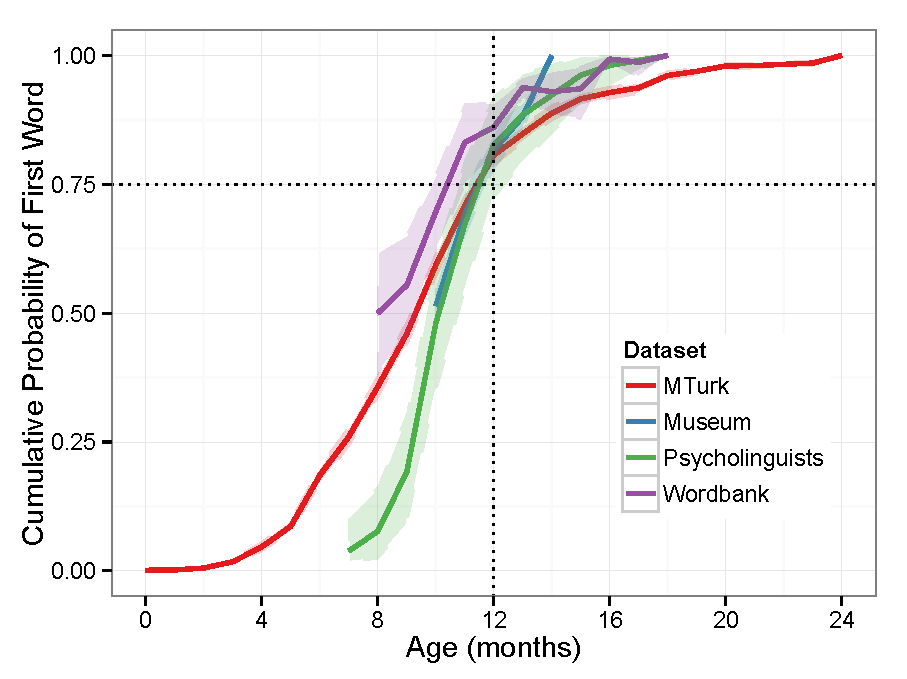
\includegraphics[width=1\linewidth]{Figure1.pdf}
\end{center}
\caption{Figure 1: Age graph showing the cumulative probability of producing a word as a function of age.}\
\end{figure}

Before 12 months, approximately 75% of children have produced a first word, and we see a gradual but consistent increase as the child ages as expected. The plot of the Mechanical Turk data, the largest dataset, is most likely the most representative of child word production, while the other datasets asymptope fairly quickly between about 14 and 17 months. 
These data suggest that children are speaking before 12 months relatively frequently. To discern whether there might be a bias on behalf of parents of older children to report a younger first word, we ran a (TEST), but did not receive a significant result (p > XX). \\
Why are some children producing language earlier than other children, and what does this reveal about the relationship between their conceptual and linguistic development? When children produce early language (<12 months) as opposed to a later one, are they choosing to produce conceptually different words than children who speak later? Or, are conceptual and linguistic development more closely linked? In our next analysis, we examined the CDI category frequencies of children's first words to explore whether very early first words differ conceptually from later-produced words. 

\subsection{CDI Categories} 
Previous work has established that the CDI normative categories are not equally represented in first word production (Fenson et al., 1994). If early word producers have a different distribution of CDI categories, this might suggest that linguistic development is loosely related to conceptual development, and that a later producer is sampling from a larger array of words that are conceptually available to her.\\
In this analysis, CDI categories were assigned by the researcher based on the MB-CDI parental report form, and validated across datasets. In instances where words did not appear on the MB-CDI,  categories were assigned ad hoc and validated across datasets for consistency. Ninety-one children were excluded because their first word was unable to categorized. We grouped the data by dataset, and performed an age split at 12 months. Figure 2 shows the frequencies of the CDI categories split by age and grouped by dataset.

%FIGURE 2
\begin{figure}[t]
\begin{center}
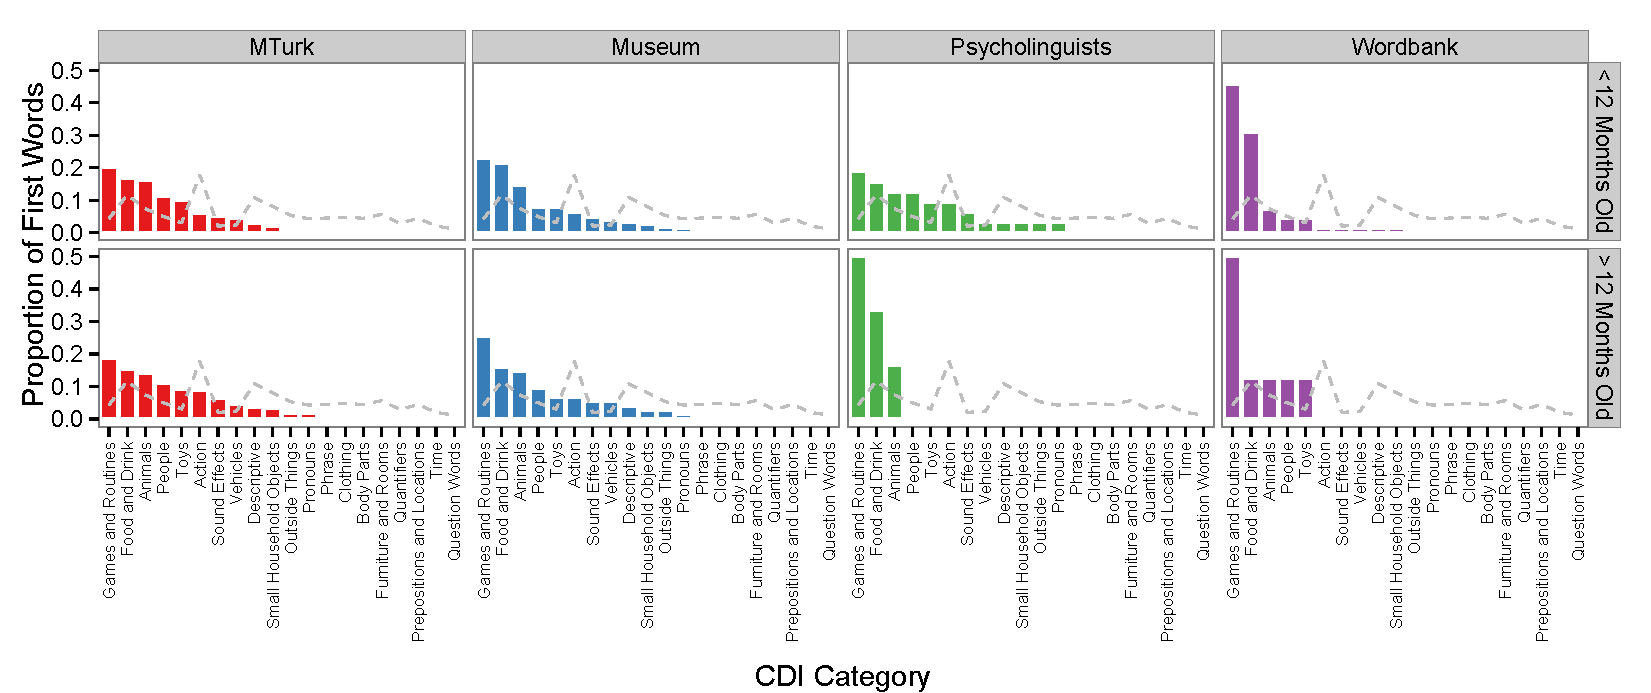
\includegraphics[width=1\linewidth]{Figure2.pdf}
\end{center}
\caption{Figure 2: Histogram of CDI category frequencies across datasets.}
\end{figure}

Distributions of CDI category frequency across all 4 datasets look quite similar. We constructed a linear model, and did not find an effect of dataset on CDI category distribution (p > XX). Although more children are included in the > 12 month group, the distributions of the CDI category representations remain very similar, as are the individual first words within the datasets (collapsed across ages, Figure 3).\\



%FIGURE 3

\begin{table}[h]
\begin{center}
\begin{tabular}{ | p{1.8cm} | p{1.8cm} | p{1.8cm} | p{1.8cm} | }
    \hline
    CDM & MTurk & Info & Wordbank \\ \hline
    Ball\newline(n = 51) & Dog\newline(n = 110) & Up\newline (n=3) & Baa Baa\newline (n=16) \\ \hline
    Hi\newline (n = 29) & No\newline (n = 108) & More\newline (n = 3) & Uh-Oh\newline (n = 7) \\ \hline
    Dog\newline (n = 29) & Ball\newline (n = 102) & Hi\newline (n = 2) & Yum Yum\newline (n = 3) \\ \hline
    Uh-Oh\newline (n = 21) & Bottle\newline (n = 76) & Cat\newline (n = 2) & Woof Woof\newline (n=3) \\ \hline
    Duck\newline (n = 16) & Hi\newline (n = 57) & Bye\newline (n = 2) & Hi\newline (n = 3) \\ \hline		
    \end{tabular}
\caption{Figure 3: Most frequent first words by dataset.}\
\end{center}
\end{table}



Animals, Games and Routines, Toys, and People, followed closely by Food and Drink are frequent first word categories, and seem to be equally compelling as a first word for both early and later producers. Data for later speakers in Wordbank is sparse, because children were selected for this analysis when they were producing exactly one word, according to parental report on the MB-CDI. Only (XX) children produced only exactly word in this group. \\
Despite producing a first word during different points in their conceptual development, both early and later producers are choosing to speak about the same semantic categories. This would suggest that children's linguistic and conceptual development are more intimately related, and the production of a first word is possibly not just the result of a cognitive shift, but an ability to produce and form words. \\
However, out of all the sets of possible first words, why are children consistently choosing to produce words predominantly from these semantic categories? What is tipping the balance in favor of these particular words? Some potential factors are frequency of parental input, the phonetic probability and ease of production, and potentially just relevance to a developing child. In the next analysis, we examine all of these within CDI categories to attempt to untangle what causes the measure of consistency we observe in first word variability.


- Describe analyses
- Details of stats- 
- Differences across studies
Consistent with previous work, we observe first words being drawn from certain CDI categories over others. We find that Animal, Games and Routines, Toy, and People words are more frequently first productions for both older and younger children, and that these patterns seem to be consistent across development. \\
These data support previous findings on CDI category analyses of early language production 
- Data suggests

\subsection{Input Frequencies}
- Question
- Describe analyses
- Details of stats
- Differences across studies
- Data suggests

\section{Discussion}

\section{Acknowledgements}




\end{document}
